\documentclass[10pt,a4paper]{article}
\usepackage[utf8x]{inputenc}
\usepackage{ucs}
\usepackage[hebrew,english]{babel}
\usepackage{amsmath}
\usepackage{amsfonts}
\usepackage{amssymb}
\usepackage{graphicx}
\usepackage{caption}
\usepackage{subfigure}


\begin{document}

\begin{titlepage}
\begin{center}

        {\LARGE Computational Fluid Dynamics Modeling of Cathodic Arc Jet in Subsonic Flow Field  \par}
         \vskip 1em
        {\LARGE \selectlanguage{hebrew}מידול זרימה חישובית של סילוני גז מקשתות קתודיות בשדה זרימה תת-קולי \selectlanguage{english} \par}
        \vskip 2em
        A Master's Thesis Proposal \\
        {\tiny by} \\
        Anton Ronis\\
        \textit{ID} \texttt{314201005}\\
        \vskip 2em
        Primary Thesis Advisor \par
        Prof.~Igal Kronhaus\par
        {\Large \makebox[3in]{\hrulefill} \par}
        \vskip 1em
        {\small
            \today \\
            Faculty of Aerospace Engineering\\
            Technion - Israel Institute of Technology\\
            Technion City, Haifa 32000, Israel\\}
    \par

% prevent a page break from being put at the end of the title page so that 
            % the contents of the paper spill onto the title page
    % save the function of the \newpage macro so we can restore it later
    \global\let\newpagegood\newpage
    \global\let\newpage\relax
\end{center}
\end{titlepage}
% restore the \newpage command after creating the title page
\global\let\newpage\newpagegood

\section{Introduction}
The quest of improving ones desired aerodynamic flow design parameters, has been initiated since the beginning of human flight. In order to try and accomplish this goal, the concept of flow-control devices has been established.
\par A flow-control device affects the original flow field, thus enabling controlling flow characteristics such as reduction of drag by delaying and/or eliminating separation zones.
The flow-control devices fall into two main categories:
\begin{enumerate}
	\item Active devices.
	\item Passive devices.
\end{enumerate}
The difference between the two categories is the usage of external energy source to control the desired flow characteristics (e.g. pumps, bleeds \textit{etc.}). Practical requirements of flow-control techniques such as robustness, light weight and ease of implementation, tend to favor passive devices such as vortex generators (VGs).\par
The concept of using VGs, first introduced by Taylor \cite{1} in the late 1940s, is based on increasing the near-wall momentum through the momentum transfer from the free-stream flow. He arranged a row of small plates/airfoils that projected normal to the surface at an angle of incidence, $\beta$, to the local flow which produced streamwise trailing vortices.\par 
Further investigations were conducted, considering the effect on pitch-up and wing-dropping problems, buffet boundary, aileron effectiveness and airplane drag for a swept-wing fighter airplane at transonic speeds, via flight tests \cite{2} showing positive results while noting no noticeable drag increase due to lift.\par
A newer approach suggests the usage of micro vortex generators (MVGs), whose height, $h$, is less than the boundary-layer thickness, $\delta$, placed ahead of a region with adverse flow conditions. In addition to the effects on subsonic flows, MVGs have been also proposed as being able to improve the adverse effects caused by shock/boundary layer interactions (SBLIs) over transonic wings \cite{3}. 
\section{Research Objectives}

In the proposed research, the effects of an array of MVGs, placed on an infinite wing, subjected to subsonic flow will be investigated. The tested MVGs will be of co-rotating vanes type, as were shown to be effective for a high energy flow \cite{1,2}. A vanes type MVGs are shown in Figure~\ref{fig:vanes}.\par
The research will focus on the following subjects:
\begin{enumerate}
%	\item \textbf{Separation zone}:\quad The detachment line distance from leading edge will be compared to the uncontrolled case. The attachment line and the total separation zone length will be compared as well.
	\item \textbf{Drag}:\quad Drag will be calculated for both controlled and uncontrolled solutions. A comparison of the drag due to lift for the two cases will be analyzed, and an attempt to evaluate the compressibility effect will be made.
	\item \textbf{Sweepback}:\quad The effect of the MVGs on swept wings will be studied. Accounting for the spanwise flow and assessing the influence o the MVGs on 3D separation regions (or process). 
%	\item \textbf{Stall Properties}:\quad Stall properties will be analyzed in the form of stall angle for both controlled and uncontrolled cases.
	\item \textbf{Flow regions}:\quad In both the 2002 review \cite{1}, as well as in the 2011 review {3} the majority of experimental studies used a bump type model placed on a flat surface. The effect of the interaction between the lower and upper streams around the wing might be interesting since in this case the separation bubble, if exists, is ``open'', thus enabling the comparison to a flow over an upper section of the wing (single domain).
\end{enumerate} 
\par
The study will be conducted by solving numerically the flow equations (NS), of a finite wing section (chunk) with periodic boundary conditions, using the freesource program \texttt{SU$^2$} and/or the proprietary program \texttt{EZNSS}. In order to eliminate turbulent-model dependence on the results, the solution will be solved using one turbulent model (SA), and the results will include an uncertainty factor (percentage) for the calculated flow characteristics for several commonly used turbulence models.
\begin{figure}[ht!]
	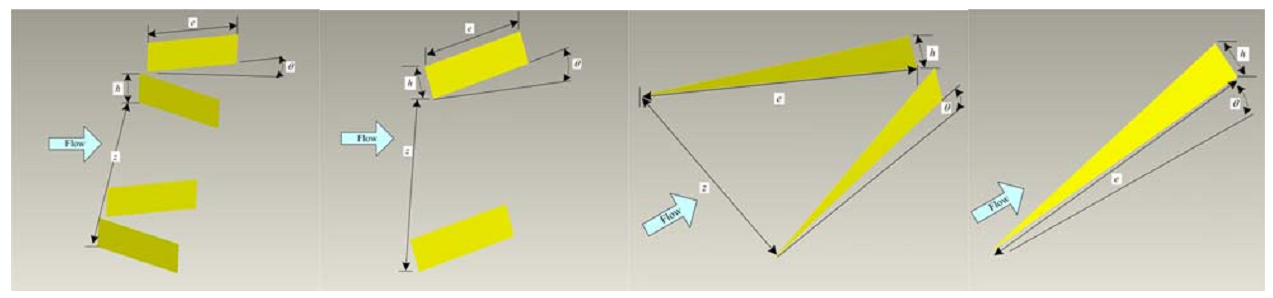
\includegraphics[width=1\textwidth]{vanes.png}
	\caption{Vane configuration \cite{3}, co-rotating and counter-rotating.}
	\label{fig:vanes}
\end{figure}

\begin{thebibliography}{99}

\bibitem{1}
  John C. Lin,
  \emph{``Review of Research on Low-Profile Vortex Generators to Control Boundary-Layer Separation``}. Progress in Aerospace Sciences Volume 38, Pages 389-420. November, 2002.
\bibitem{2}
  Norman M. McFadden,George A. Rathert,Jr. and Richard S. Bray,
  \emph{``The Effectiveness of Wing Vortex Generators in Improving the Maneuvering Characteristics of a Swept-Wing Airplane at Transonic Speeds``}. National Advisory Committee for Aeronautics, Technical Note 3523, Ames Aeronautical Laboratory. Moffett Field, California. September, 1955.
\bibitem{3}
Frank K. Lu, Qin Li, Yusi Shih, Adam J. Pierce and Chaoqun Liu,
  \emph{``Review of Micro Vortex Generators
in High-Speed Flow``}. 49th AIAA Aerospace Sciences Meeting. Orlando, Florida. 4 - 7 January, 2011.

\end{thebibliography}

\end{document}
